% target: 6 pages
\mychapter{1}{CHAPTER 1. INTRODUCTION}\label{ch:chap1}
\graphicspath{{./chapter1/image/}}

Recommendation systems have been applied in a vast range of industries, ranging from retail to healthcare, and it is undoubtedly getting more and more popularized in the next few decades. Many recommender systems leveraged by artificial intelligence has reinforced users’ selection and brings about superhuman solutions. In such a background, a hair and clothes color recommendation system that helps them select the most suitable color is in desire of society.  Hair and cloth segmentation models are addressed as the core of this thesis; they, in this study, are proposed and assessed. From that, the thesis proposes a prototype for beauty apps, including use-case analysis, interface and architecture design. Afterward, real-time hair and cloth recoloring application for mobile devices is developed and finally evaluated. \par

\section{Motivation}
It is true that the clothing industry is in the top-4 most lucrative fields and often accounts for a significant portion of personal expenditures. People nowadays want to look good and expect higher at their outfits as the standard of living rises across the world. As a result, many find their preferred models, cuts, and styles of clothing but do not know what colors are the most well-suit to buy. These colors must flatter your skin tone or match with accessories’ tones. For a good outfit, pieces of clothes should not have any pair of complementary colors such as blue vs. orange, red vs. green. Usually, these color theories are well understood by stylists and fashionistas.
\par
Nevertheless, in case they choose a wrong color, many consequences might arise from that. Clothing that is not preferable is less likely to be worn, or more seriously, be discarded. Furthermore, it would form consumerism among society when people have not figured out suitable outfits, consequently increasing our environmental footprint. According to a report, the apparel industry's environmental impact, which is calculated throughout the entire life cycle of clothing, occupied 20\% of global water waste and 10\% of global carbon emission \cite{carbonemission}. Selecting clothes color visually on mobile phones is incredibly beneficial to the fashion industry.\par

Both women and men wear their hair in a variety of styles; each haircut can be dyed to many colors. With a multitude of colors, people always are often confused about commit a color from the wide variety available to them. 
\par
Considering the reasons mentioned earlier, there exists a need for a beauty app that helps the client to save time and effort in choosing hair and clothes color. Additionally, hair segmentation information can not only advance recommendation systems, but it is also used for a variety of applications, such as photo editing, make-up changes, and face detection. Further uses of clothing segmentation information appear on virtual try-on, clothing retrieves system, all of which are valuable applications for everyone in daily life.
\par
\section{Problem background} \label{sec:pb}

Augmented reality is an emerging technology, and it provides users with an interactive experience in both the physical and digital worlds. An augmented reality system aims at creating a real-time modification of the real-world environment for an interactive experience. Augmented reality continues to proliferate and become pervasive among a wide range of applications, including beauty. In the beauty industry, where live virtual try-on of beauty products is of great importance, augmented reality involves overlaying visual information onto real scenes so that not only user’s experience enhances, but companies also promote their products. To advance this domain, the segmentation task plays a key role.
\par
Semantic image segmentation, the task of mapping each pixel to a label, is a major and old challenge in the area of computer vision. Image segmentation can be treated as pixel-level prediction because it classifies each pixel into its category. With hair, segmentation problem strives for even fine details of strands of hair and avoid confusion between skin and hair. In the clothes segmentation problem, the output is a semantic analysis showing which clothing items are present, where in the image these are, and what shape they have.

\begin{figure} [H]
    \centering
    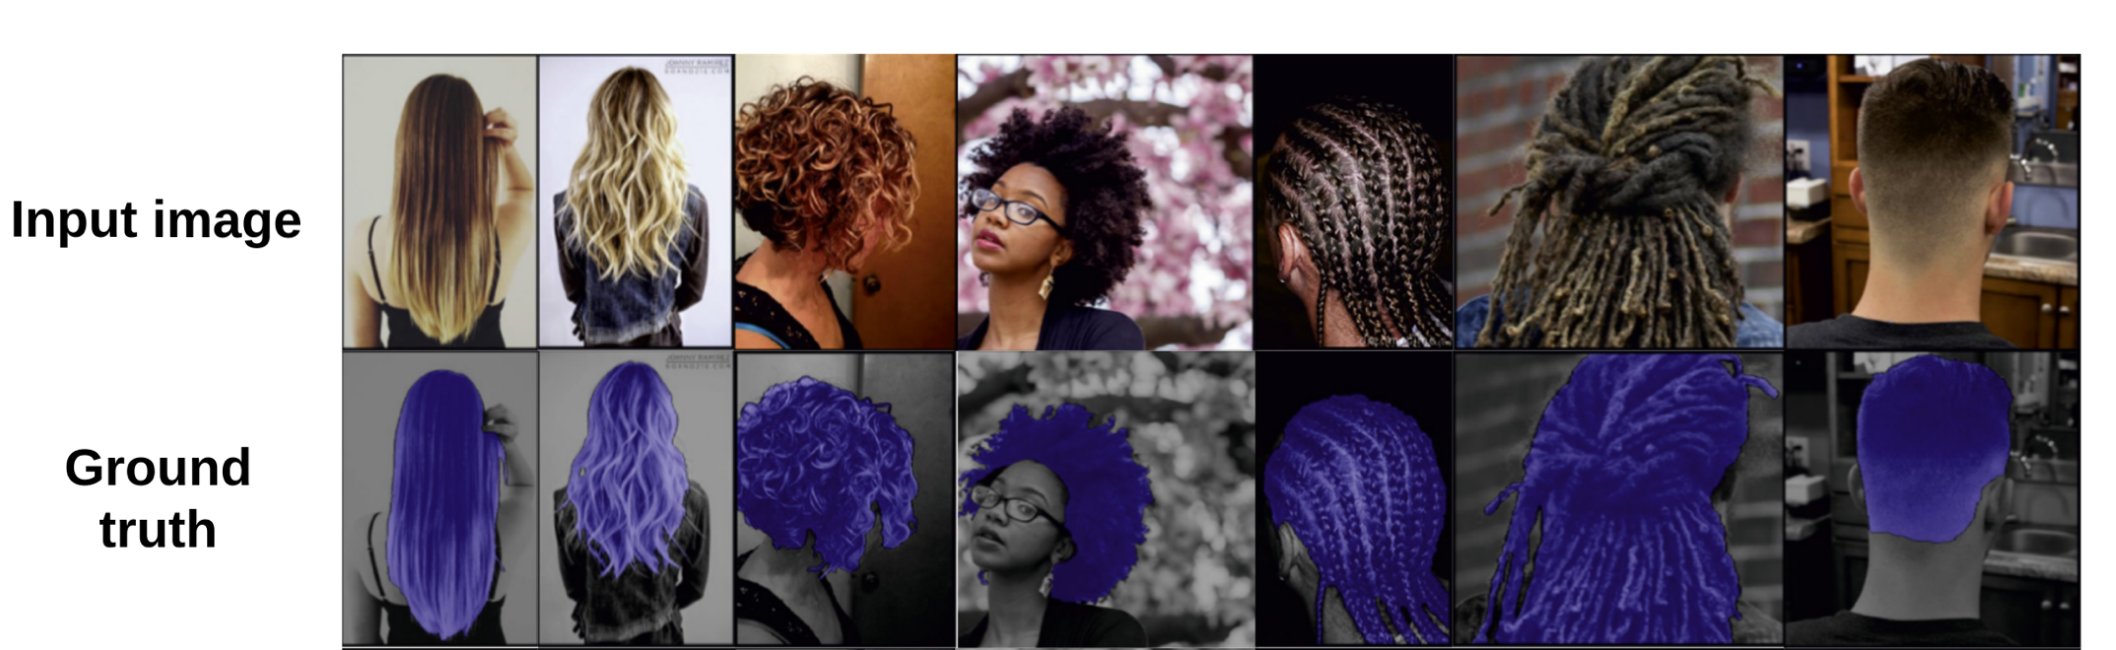
\includegraphics[width=0.9\textwidth]{chapter1/image/hair seg.png}
    \caption{Illustration for hair segmentation task. Hair masks is blue in color.}
    \label{fig:c1hairseg}
\end{figure}

With deep learning applied, this problem has been on the way to get an advanced performance in understanding image data. In addition to accuracy, the extent of media has also been extended to cover not just 2D images but also 3D images, videos, and so on. Apart from that, the field of deep learning possesses active communities and professional support. Tools for developing deep learning applications, such as Tensorflow, PyTorch, Caffe, were built in a modular way with a thorough document that makes development and engineering much more efficient. 
\par

Prior to the deep learning revolution, traditional image processing algorithms were used for both hair and clothes segmentation, but with deep learning, features are obtained automatically. Recent DNNs for hair segmentation are FPN \cite{fpn}, DenseNet \cite{densenet}, DeepLabv3 \cite{deeplabv3}. Aside from architecture, a hair matting technique utilizing image gradient is introduced in \cite{hairseg2matting}, playing the role of an auxiliary loss. Researchers also make an effort to apply filters to treat coarse masks \cite{hairseg2matting}. About clothing segmentation problem, Mask R-CNN \cite{maskrcnn}, Match R-CNN \cite{deepfashion2} are proposed to achieve instance segmentation in spite of complex architecture. The thesis work will exploit the start-of-the-art solution for hair and cloth segmentation tasks to achieve the thesis's goals. 
\par
\paragraph{Problem of real-time segmentation on mobile devices}

DNNs for segmentation are complex and require high memory usage and computational resources. Therefore, the main platforms to run these models must have a powerful computational unit (e.g., GPU support) or cloud. For instance, mobile applications often send input and receive output from Firebase, where developers push their DNNs. However, researchers recently realize the benefits of bringing deep learning toward the edge that includes devices with less power and resources. It ranges from user experience, offering anytime, anywhere access, with the great advantages of security, privacy, and energy consumption. \par

Discovering advantages from running DNNs on edge, big technology companies have been developing more and more frameworks to deploy models locally. A few must-mentioned frameworks for deep learning on mobile phones are TFLite, OONX, CoreML, PyTorch Mobile. Almost all frameworks for smartphones concern about optimization level, binary size, and supported hardware. Take the QNNPACK library \cite{qnnpack} for example, it is a mobile-optimized library for low-precision high-performance neural network inference. QNNPACK also provides the implementation of common neural network operators on quantized 8-bit tensors. Moreover, models developed especially for mobile also raise in the number; some of them are introduced in \textbf{section \ref{sec:cnn}}. 




\section{Objective and Contributions}

The thesis focuses on creating an Android app for the beauty field, aiming at smoothness and efficiency. By providing a real-time interaction experience, users see immediate feedback on objects they are tracking (at here are hair and clothes). In detail, users can preview images taken from cameras with hair or clothes being recolored and select a color as they like. Afterward, users are able to save or share images with hair and clothes recolored into storage. As a part of this thesis study, it is to research two crucial components: a fast on-device running model and a well-designed mobile app. Later, the problem in combining these two components is also seriously raised and tackled in my thesis. All in all, real-time performance on a wide variety of mobile devices is prioritized, while pixel-perfect masks may not be provided. \par
There are two main contributions of the thesis: a real-time beauty camera app running on Android and two deep learning models adapted for smartphones. About the app, it is designed with ten basic use cases, two of them are main features, namely Clothes Camera and Hair Camera. The real-time camera based on the CameraX framework achieves the speed of 60 FPS. In terms of masks rendering, I propose two methods (Bitmap and OpenGL), bringing about a good enough user experience. For rendering hair and clothes masks, it takes 24ms with OpenGL and slower with Bitmap. About the hair and clothes segmentation models, these two models achieve  86\% IoU on average. \par
\section{Difficulties} 
Hair can be classified into many categories, light or dark, curl or straight, etc. Therefore, many hair segmentation models can recognize hair in black or yellow but fail to the other colors. In addition to multiple variants, hair has an unstable and complex structure, unlike many objects with simple shapes. In terms of clothing, the color and shape of it are also incredibly various. Covering all these possibilities will lead to hardship in hair and clothing recognition, which ought to be resolved in the thesis work.


Nevertheless, smartphones usually constrain the memory of 4 gigabytes in total; thus, standard models would consume a large proportion of memory space. Also, long inference time of standard models is problematic, although hardware accelerators come into handy. One other difficulty in running models on mobile devices is that the size of the output mask is different from the size of the screen. Because of this mismatch, we have to rescale and meticulously render predictions to fit the screen. Furthermore, it is also essential to ensure that pipelines runs consistently on targeted environments and produces identical results with the inputs stay the same. 



\section{Thesis structure}

There are totally five chapters in this thesis proceeded as follows. \par 
\textbf{Chapter 1: Introduction.} This chapter gives an overview of the thesis work, presents reasons and motivations of the work. Besides, some lately advancements in the field of semantic learning, smartphone deployment is briefly introduced. After this chapter, readers get a view of difficulties in hair and clothes segmentation, aside from objectives that the thesis follows.  \par
\textbf{Chapter 2: Background.} This chapter firstly introduces some convolutional neural networks that have been deployed on mobile devices, along with their specific applications. Secondly, Android and a few libraries are presented; it is also mentioned the reasons why they are used. Finally, tools for model deployment are given basic understand with TFLite is the core. TFLite is described with model optimization and converter.  \par
\textbf{Chapter 3: Method.} 
This chapter explains the architecture of the proposed model, the app pipeline. For the DNN, it is also explained the reasons why the architecture is chosen. For the app, we provide a brief introduction of hardware accelerator and TFLite backend support. At last, two rendering methods are presented. \par
\textbf{Chapter 4: Experiments and Result.} This chapter indicates experiments conducted on both the app and the model, gives quantitative results after that. Finally, this chapter concludes the thesis and suggests future work.\par